\documentclass{article}
\usepackage{epsfig}
\usepackage{graphicx}
\usepackage[table]{xcolor}
\usepackage{tikz}
\title{CS345 Theoretical Assignment 1 \\ }
\author{\vspace{2mm} \large Ayush Agarwal, 13180 \\ M.Arunothia, 13378}
\date{}
\begin{document}
\maketitle
\tableofcontents
\newpage
\section{Non-Dominated Points}
\subsection{Overview}
Given a set of coordinates P, we create list of each layer in the following manner.\\
First sort the coordinates based on Y-coordinate in descending order. Then maintain an array A of size $n$. Start with the first coordinate from 
the sorted array P(of all coordinates). This point will be a non-dominated point and will be a part of layer 1. Update the first index of A with the x-coordinate
of this point. Now take the second point from P. If its x coordinate is greater than the x-coordinate of earlier point, it means that it will be part of layer
1. If so then add it to layer 1 and update the layer 1's index in A. Otherwise it will be in second layer, so add it in layer 2 and update the layer 2's index 
in A with it's x coordinate. Repeat the above procedure for all points.

\subsection{Pseudo-Code}
Non-Dominated-points(P)	\\*
\{			\\*
    \hspace*{1cm}$ P  \longrightarrow  reverse\_sort(P)$ //sort in descending order of Y  \\*
    \hspace*{1cm} $ Layer[n]; A[n] $\\*
    \hspace*{1cm} $ A[0]=P[0].x $\\*
    \hspace*{1cm} $Layer[1].push()$ \\*
	\hspace*{1cm} $i=1; right=1 $\\*
    \hspace*{1cm} $while(i < P.length())$\\*
    \hspace*{2cm} $point = P[i]$\\*
    \hspace*{2cm} $index = binary\_search\_predecessor(A, 0, right, point)$ \\*
    \hspace*{4cm}                // returns the predecessor's index \\*
    \hspace*{2cm} $Layer[index].push(point)$\\*
    \hspace*{2cm} $A[index] = point.x$\\*
    \hspace*{2cm} $If (index > right ) right++ $\\*
	\hspace*{1cm} $return  Layer $\\*
	\\*
\}
\subsection{Time Complexity}
  Sorting step takes $O(nlogn)$ time, followed by binary\_search for each point which takes $ logn $ time per point.
  While iterates for all the points and in each iteration binary\_search is invoked, thus the loop takes $ n*logn $ time.
  Overall algorithm takes time \\
             $O(nlogn) + O(nlogn) = O(nlogn) $
\subsection{Proof of Correctness}
!!!Not written!!!
\newpage
\section{ Open Rectangle Query }
\subsection{Data Structure Design : } 
Given an array 'a' of 'n' coordinate points, we construct a Binary Search Tree (BST) call it 'data' in the following manner.\\*
\begin{itemize}
\item Sort the array 'a' w.r.t the x-coordinates of the points. Call this sorted array 'b'.
\item Divide 'b' into $ \frac{n}{Log[n]} $ parts, starting from the beginning. Index each of the part incrementally from 1 to $ \frac{n}{Log[n]} $. 
\item Construct BST 'data' with $ \frac{n}{Log[n]} = N $ nodes from 'b' using the above indexing for the comparisons.
\item Now, we have a BST 'data' with 'N' nodes augmented with an array of $Log[n]$ size at every node. Sort this array at every node on basis of y-coordinates of the points.
\item This completes the description of augmented BST 'data'.
\end{itemize}
\section*{Given Array 'a'}
\hspace{-4.8cm}
\begin{tabular}{ |c|c|c|c|c|c|c|c|c|c|c|c|c|c|c|c|}
\hline
\cellcolor{red} (13,1) & (4,2) & (11,3) & (2,4) & \cellcolor{red} (8,5) & (9,6) & (5,7) & (14,8) & \cellcolor{red} (3,9) & (12,10) & (10,11) & (6,12) & \cellcolor{red} (1,13) & (16,14) & (15,15) & (7,16) \\ \hline
\end{tabular}
\section*{Sorted Array 'b' based on x coordinates}
\hspace{-4.8cm}
\begin{tabular}{ |c|c|c|c|c|c|c|c|c|c|c|c|c|c|c|c|}
\hline
\cellcolor{red} (1,13) & (2,4) & (3,9) & (4,2) & \cellcolor{red} (5,7) & (6,12) & (7,16) & (8,5) & \cellcolor{red} (9,6) & (10,11) & (11,3) & (12,10) & \cellcolor{red} (13,1) & (14,8) & (15,15) & (16,14) \\ \hline
\end{tabular}
\section*{BST 'data' constructed for this example}
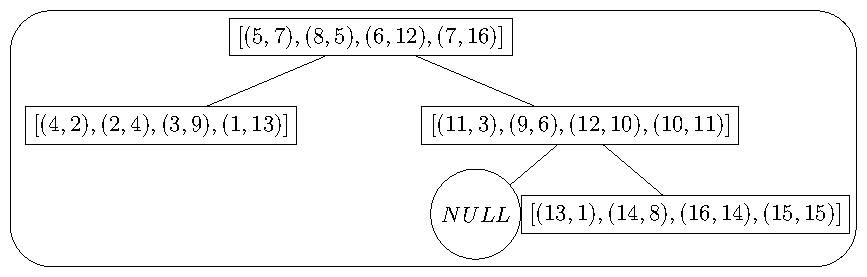
\includegraphics[scale=1]{bst.pdf}
\subsection{Algorithm : }
\begin{itemize}
\item[\bf STEP 1 : ]
Start
\item[\bf STEP 2 : ]
If($x_2 - x_1 < 2*(Log[n]) $, traverse elements in this range of x and return the points satisfying $y > y_{bottom}$. \\*
else Initialise variables node\_i to the x value of nearest node ahead of $x_1$ and node\_j to the x value of nearest node behind $x_2$.
\item[\bf STEP 3 : ]
Find the elements satisfying $y > y_{bottom}$ in the x range $x_1$ to node\_i and in x range node\_j to $x_2$, and report them.
\item[\bf STEP 4 : ]
Find the elements satisfying $y > y_{bottom}$ in the x range node\_i to node\_j and report them.
\item[\bf STEP 5 : ]
Stop.
\end{itemize}
\subsection{Pseudo Code : }
Report\_points($x_1,x_2,y_bottom$)	\\*
\{			\\*
	\hspace*{1cm}if($ x_2-x_1 <2*(Log[n])$) \\*
	\hspace*{2cm} Locate the required x range in the BST. \\*
	\hspace*{2cm}Report elements between that x range satisfying $y > y_{bottom}$ using binary search \\*
	\\*
	\hspace*{1cm}else if($x_1$ and $x_2$ exists in data points)\\*
	\hspace*{2cm} Locate the required x range in the BST. \\*
	\hspace*{2cm}Report elements between that x range satisfying $y > y_{bottom}$ using binary search \\*
	\\*
	\hspace*{1cm}else \\*
	\hspace*{1cm}node\_i $ \longrightarrow $ x value of the nearest node ahead of $x_1$ \\*
	\hspace*{1cm}node\_j $ \longrightarrow $  x value of the nearest node before $x_2$ \\*
	\hspace*{1cm}report\_i $ = $ Report\_points($x_1$, node\_i, $y_{bottom}$)		\\*
	\hspace*{1cm}report\_j $ = $ Report\_points(node\_j, $x_2$, $y_{bottom}$)		\\*
	\hspace*{1cm}report\_rest $ = $ Report\_points(node\i, node\j, $y_{bottom}$)		\\*
\}	 
\subsection{Space Complexity : }
	The data structure we invented, is a BST of size N*(augmentation size).\\*
Therefore, space used is $N * Log[n]$= n. (Refer Sub section Data Structure Design).
Implying space complexity is O(n).
\subsection{Time Complexity : }
\subsubsection{Query Time : }
!!!Not written!!!
\subsubsection{Pre-processing Time : }
\begin{itemize}
\item The first sort based on x coordinates requires O(n*Log[n]).
\item 
\item
\item

\end{itemize}
\subsection{Proof of Correctness}
!!!Not written!!!
\newpage
\section{Constraint of each commando}
\subsection{Overview}
This problem is approached using the divide and conquer strategy. As the square dimension is in powers of 2, we can divide the square we get in every iteration into 4 squares of equal size. Let 'P' = p(x,y) be the coordinates of Prime Minster's cabin. Define a recursive function Report(Square,n,P) which works by divide and conquer. Where 'Square' gives the square boundaries and 'n' gives its side length. 
\subsection{Algorithm}
\begin{itemize}
\item Start.
\item {\bf if($n<2$)} return with reporting "No points"
\item {\bf else if($n==2$)} return position of commando as the one diametrically opposite to P in the square. Orientation will be facing P so that he can cover the L-shape leaving out Prime minister's office.
\item {\bf else} divide the square into four equal squares of side length n/2. $P_1$, $P_2$, $P_3$ and $P_4$ are estimated as follows. The quadrant that has P currently will retain it as its $P_1$ and this square is called ${Square}_1$. The other three quadrants will have their $P_i$ to be the point that is diametrically opposite to the only corner that they have of the bigger square. where $ i \in \{2,3,4\} $.
\item Report(n,P,Square) = Report(n/2,$P_1$,${Square}_1$) + Report(n/2,$P_2$,${Square}_2$) + Report(n/2,$P_3$,${Square}_3$) + Report(n/2,$P_4$,${Square}_4$) + the commando position and orientation who can cover $P_2$, $P_3$ and $P_4$. 
\item Stop.
\subsection{Pseudo Code}
Report(n,P)	\\*
\{			\\*
	\hspace*{1cm}if($n<2$) \\*
	\hspace*{2cm} print "No Commandos required". return \\*
	\\*
	\hspace*{1cm}else if($n==2$)\\*
	\hspace*{2cm}Return Position =  diametrically opposite point to P. \\*
	\hspace*{2cm}and Orientation = direction facing P. return\\*
	\\*
	\hspace*{1cm}else \\*
	\hspace*{2cm}$P_1$ = P and ${Square}_1$ is the corresponding Square.\\*
	\hspace*{2cm}Find ${Square}_i$ and $P_i$ as defined above.where $ i \in \{2,3,4\} $.\\*
	\begin{center}
	Report(n,P,Square) = Report(n/2,$P_1$,${Square}_1$) + Report(n/2,$P_2$,${Square}_2$) + Report(n/2,$P_3$,${Square}_3$) + Report(n/2,$P_4$,${Square}_4$) + the commando position and orientation who can cover $P_2$, $P_3$ and $P_4$. \\*
	\end{center}
	\hspace*{1cm}return \\*
\}
\subsection{Time Complexity}
\begin{center}
$ T(n) = 4*T(n/2) + a $ \\*
$ = 4^{log(n)} + constant $ \\*
$ = O(n^2) $ \\*
\end{center}
\subsection{Proof of Correctness}
\subsubsection{What is to be proved? or Claim}
That given any square of side length 'n' (a power of 2)  and Prime Minister's office P we can exhaust the rest of the square with non overlapping pieces of L-shaped tiles ( L-shape containes 3 unit sqaures and hence is equivalent to the given problem).  \\*
\subsubsection{Proof by Induction}
Induction is carried out on the length of the square. \\*
\subsubsection{Base Cases}
\begin{itemize}
\item $(n<2)$ - No commandos needed. \\*
\item $(n==2)$ - Only one commando needed and he should be placed so as to cover 'L' shape that leaves out Prime Minister's cabin. \\*
\end{itemize}
\subsubsection{Hypothesis}
Let $ n = 2^{k} $. \\*
Let us assume that the Claim is true for all $i<=k$ where $k>2$ and both are integers. \\*
\subsubsection{Inductive Step}
Let us prove that claim for $ k+1 $ is true. \\*
The square of size $2^{k+1}$ can be broken into four squares of size $2^{k}$. As the claim holds for sizes $<=k$, these 4 squares can be exhausted in the required way, (i.e) PM cabin anywhere we chose it to be and the rest exhausted with non overlapping 'L' shapes. \\*
\begin{center}
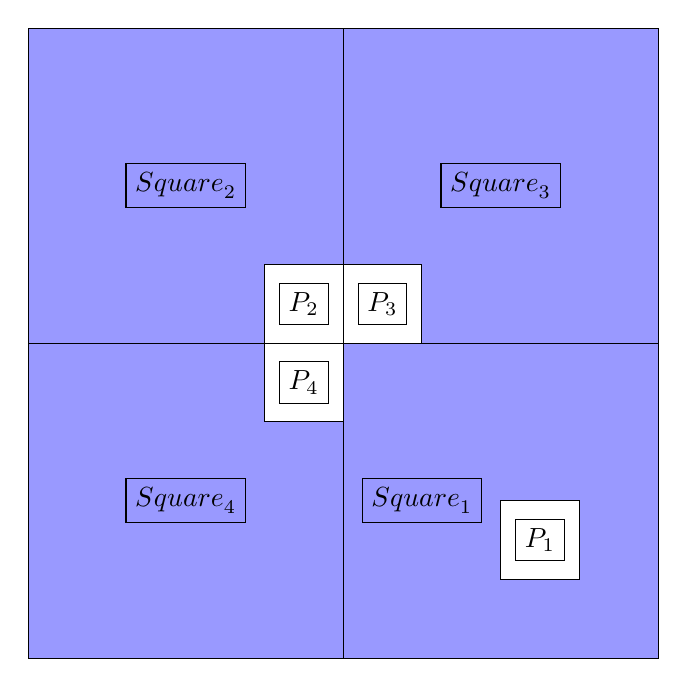
\begin{tikzpicture}
\draw[step=1cm,gray,very thin] (-2,-2) grid (6,6);
\filldraw[fill=blue!40!white, draw=black] (-2,2) rectangle (2,6);
\filldraw[fill=white, draw=black] (2,2) rectangle (1,3);
\filldraw[fill=blue!40!white, draw=black] (2,2) rectangle (6,6);
\filldraw[fill=white, draw=black] (2,2) rectangle (3,3);
\filldraw[fill=blue!40!white, draw=black] (-2,2) rectangle (2,-2);
\filldraw[fill=white, draw=black] (2,2) rectangle (1,1);
\filldraw[fill=blue!40!white, draw=black] (2,2) rectangle (6,-2);
\filldraw[fill=white, draw=black] (4,0) rectangle (5,-1);
\node[draw] at (1.5,2.5) {$P_2$};
\node[draw] at (2.5,2.5) {$P_3$};
\node[draw] at (1.5,1.5) {$P_4$};
\node[draw] at (4.5,-0.5) {$P_1$};
\node[draw] at (0,4) {${Square}_2$};
\node[draw] at (4,4) {${Square}_3$};
\node[draw] at (0,0) {${Square}_4$};
\node[draw] at (3,0) {${Square}_1$};
\end{tikzpicture}
\end{center}
Then chose, the PM cabin's as shown above. This way just by adding one more commando, on $p_2$ facing towards ${Square}_1$, we can exhaust our required full square! \\*
Thus, proved by induction. \\*
Note, this has to be an optimal solution as we are ensuring that every box is guarded by just one commando (this is because of the combine step which does not disturb any guarded box and the base case for which the claim holds). 
\end{itemize}
\end{document}
